
	\subsubsection{Use-Case Instance - uciSimpleAndCompletePart02:suDeployAndRun}
	
	Second part of a simple and complete use case instance for the summary use case \msrcode{suDeployAndRun} illustrating a simple and complete interaction scenario primarily handled by an administrator in a concrete situation. 
	\begin{operationmodel}
	\addheading{summary Use-Case Instance}
	\adddoublerow{Instantiated Use Case}{suDeployAndRun}
	\adddoublerow{Instance ID}{uciSimpleAndCompletePart02}
	
	\addrowheading{Remarks}
	\addalphanumberedsinglerow{}{starts when the coordinator logs in the system until the full handling of all the existing crisis.}
	\addalphanumberedsinglerow{}{shows an instantiated case of handling of a crisis by a coordinator until its closure after reporting.}
	\end{operationmodel} 

	
	Figure \ref{fig:lu.uni.lassy.excalibur.examples.icrash-RE-UC-uci-suDeployAndRun-uciSimpleAndComplete-Part02}
	shows the sequence diagram representing the second part of a simple and complete use case instance for the summary use case \msrcode{suDeployAndRun}.
	
	\begin{figure}[htbp]
	\begin{center}
	
	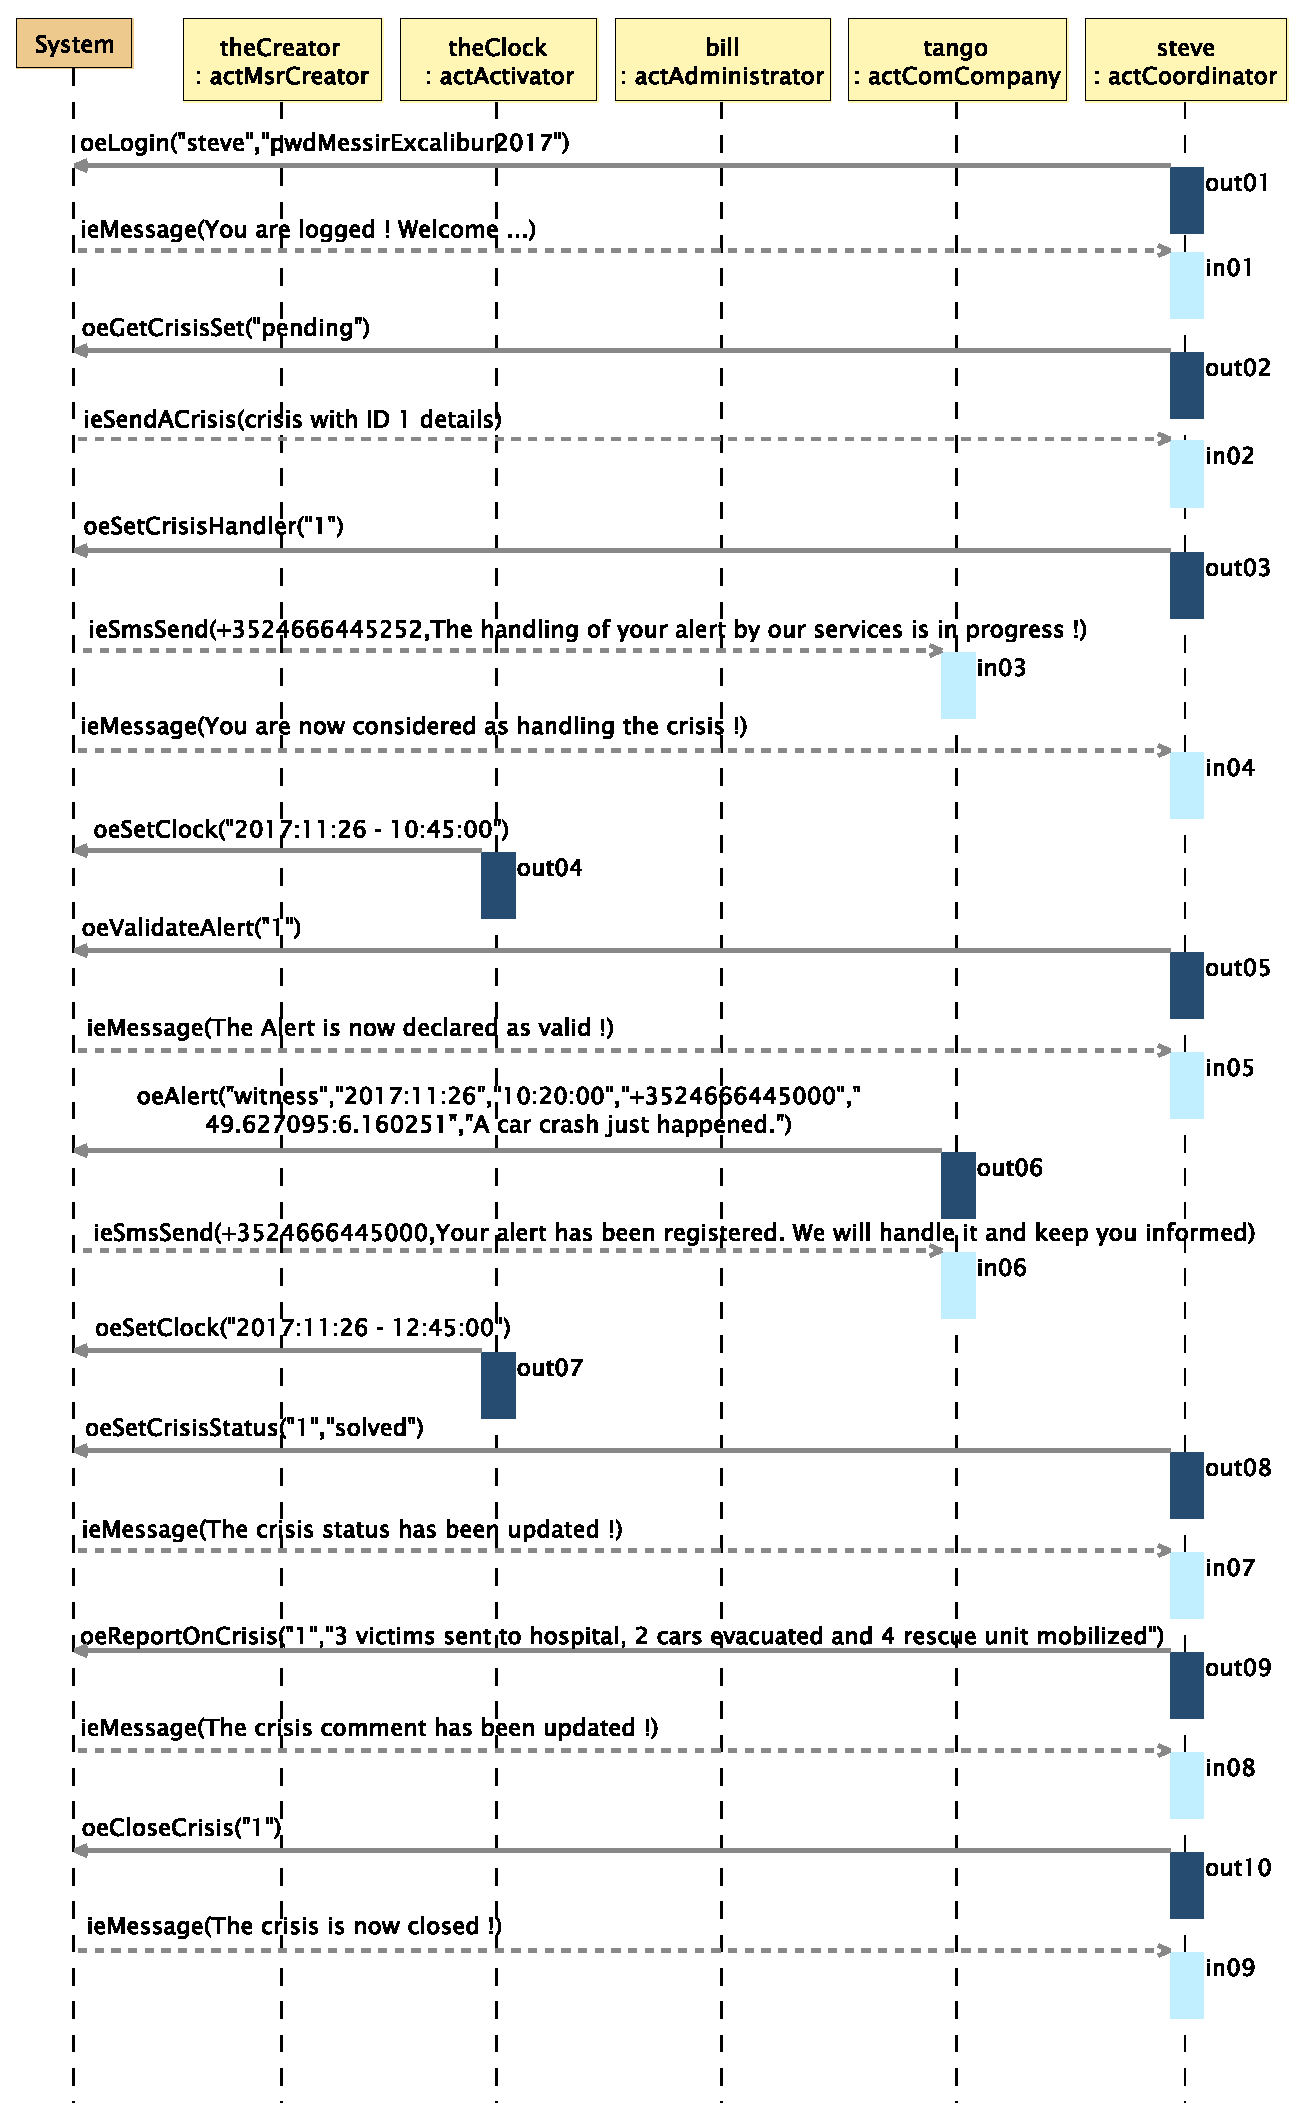
\includegraphics[
	angle=0
	,height=1.0\textheight
	]{./images-report-gen/usecase-model/summary/uci-suDeployAndRun-uciSimpleAndComplete-Part02.eps}
	\end{center}
	\caption[lu.uni.lassy.excalibur.examples.icrash Sequence Diagram: uci-suDeployAndRun-uciSimpleAndComplete-Part02]{uci-suDeployAndRun-uciSimpleAndComplete-Part02 use case instance sequence diagram
	}
	\label{fig:lu.uni.lassy.excalibur.examples.icrash-RE-UC-uci-suDeployAndRun-uciSimpleAndComplete-Part02}
	\end{figure}
	\vspace{0.5cm}
